\documentclass[a4paper,10pt]{article}

\usepackage{amsmath,mathrsfs,amssymb} % amsmath crashes with tsfonts for the command \iint
\usepackage{cmbright}
\usepackage{eurosym}
\usepackage{graphicx,subfigure}
\usepackage[usenames]{color}

\ifx\pdfoutput\undefined
\usepackage[dvipdf,
            pdfstartview=FitH,
            bookmarksnumbered=true,
            bookmarksopen=true,
            colorlinks=true,
            linkcolor=blue,
            citecolor=blue,
            filecolor=blue,
            urlcolor=blue,
            ]{hyperref}
% %%\AtBeginDvi{\special{pdf:tounicode GBK-EUC-UCS2}}} % GBK -> Unicode
\else
\usepackage[dvipdfm,
            pdfstartview=FitH,
            bookmarksnumbered=true,
            bookmarksopen=true,
            colorlinks=true,
            linkcolor=blue,
            citecolor=blue,
            filecolor=blue,
            urlcolor=blue,
            ]{hyperref}
\fi

\setlength{\parskip}{1.ex plus .2ex minus .5ex}
\renewcommand{\baselinestretch}{1.2}
\def\nuc#1#2{\relax\ifmmode{}^{#1}{\protect\text{#2}}\else${}^{#1}$#2\fi}
\renewcommand{\textfraction}{0.15}
\renewcommand{\topfraction}{0.85}
\renewcommand{\bottomfraction}{0.65}
\renewcommand{\floatpagefraction}{0.60}

\usepackage[top=2.5cm,bottom=2.5cm,left=2cm,right=2cm]{geometry}
\usepackage{makeidx}
\makeindex

\title{ActarSim Manual}
\author{H. Alvarez Pol and D.Y. Pang}
\date{\today}
%
%\listoffigures
%\listoftables

\begin{document}
\graphicspath{{figures/}}
\maketitle

\begin{abstract}
A manual for ActarSim.
\end{abstract}

\tableofcontents

\section{Introduction}
ActarSim is a code developed for the simulation of the ACTAR experimental setup.

\section{Installation}

\subsection{Requirements}

The following software components are required:

\textbf{GEANT4} - due to the physics definitions, only 4.8.0 and later geant4 versions could be used with this ActarSim simulation. It should be compiled following the instructions provided by the geant4 collaboration ( \url{http://geant4.web.cern.ch/geant4/} ). Check the installation\index{installation} with the included geant4 examples.

\textbf{ROOT} - tested on versions 5.06 and some of the latests and the old 4.03. It is mandatory to install the libraries and include directories. Follow the typical installation as shown in \url{http://root.cern.ch}.

\textbf{G4UIROOT} - not required, but very useful user interface, mainly for beginners because of their fast and painless access to the commands. Download the code from \url{http://i.home.cern.ch/i/iglez/www/alice/G4UIRoot} and follow the instructions for installation. Check the installation with the modified geant4 examples.

\textbf{ActarSim} - the present code.

\subsection{Installation}

It is recommended to take the code from the subversion repository\index{subversion repository} using the \textit{subversion} tools. Subversion is available for most of the operative systems, allowing the access to the repository where the code is stored. The required login and password combination could be obtained from the code developers (mail to repository developer, \url{hector.alvarez@usc.es}).

In case you have no access to the repository, it is possible to download an stable version of the code ActarSim\_DATE.tar.gz file on your GEANT working directory. Unpack the file with the commands:
\begin{verbatim}
        tar -xzf ActarSim_DATE.tar.gz
\end{verbatim}
A directory ActarSim will be created with the relevant files in.

In any case, after getting the code, one should compile it. To do this, enter in the ActarSim directory 
and compile it by typing:
\begin{verbatim}
        cd ActarSim
        gmake
\end{verbatim}

\subsection{Run the program}

Provided the code was successfully compiled, the code runs using the code name alone (for interactive session) or with a macro name (for a batch session):
\begin{verbatim}
        ActarSim                    // interactive session
        ActarSim batch1.mac         // batch session
\end{verbatim}

Description of the commands which can be used in the macro is given in section \ref{sec-messengers}. It would be useful to specify the terms \textit{number of events}\index{number of events} (or \textit{number of Geant4 events}) and \textit{number of reactions}\index{number of reactions} here for the following text. ActarSim calculates information of one \textit{reaction} by issuing two geant4 \textit{events}: one for the beam and a following one for the reaction products (\textit{primaries} in the glossary of Geant4). Since the event numbers in Geant4 start from zero, the \textbf{even events correspond to beams and odd events correspond to reaction products}. Having this in mind is important to understand the analyzing macros described in the following sections. Because of this, if a user wants to simulate, say, 100 reactions, he/she has to pass a number 200 to the command \textit{/run/beamOn}:
\begin{verbatim}
        /run/beamOn 200
\end{verbatim}
Another thing is that by some reason not known right now, silicon and scintillator information defined in classes \textit{ActarSimSilHit} and \textit{ActarSimSciHit}, respectively, for the $i$th reaction are written, instead in the $(2i+1)$th event, in the ($2i$)th event ($i$ starts from zero), so if the user really care about the information of the last reaction, for exampke, the 100th reaction in the previous example, he/she has to pass the number 201 to the command \textit{/run/beamOn}:
\begin{verbatim}
        /run/beamOn 201
\end{verbatim}
Of course it does not matter much if we loss information of one reaction if we simulate 10000 reactions.

\section{A typical session with ActarSim}
A typical ActarSim session\index{ActarSim session} contains the following procedures:
\begin{enumerate}
 \item Run ActarSim, in this step, the
 \item Run the digitizationMacro
 \item Run the analyzing macro
 \item Run the Ntuple\index{ntuple} reader to analysis the results
\end{enumerate}

\subsection{Running ActarSim}
An example of macro file needed to run ActarSim is given in section \ref{sec-ActarSim-macro}. Detailed explanations of the commands in this macro file are given in section \ref{sec-messengers}. Most of the commands and their parameters can be kept the same as in this example. The information that has to be provided by the user are the following:

\begin{enumerate}
\item The geometry\index{geometry} of chamber. Note that the numbers are \textit{half lengths} of the real geometry, for example, for a cubic chamber of $300\times300\times300$ mm$^3$, the corresponding commands are:

  \begin{verbatim}
  /ActarSim/det/gasGeoIncludedFlag on
  # if box
  /ActarSim/det/gas/setDetectorGeometry box
  /ActarSim/det/gas/setXLengthGasBox 150. mm
  /ActarSim/det/gas/setYLengthGasBox 150. mm
  /ActarSim/det/gas/setZLengthGasBox 150. mm
  \end{verbatim}

\item To include silicon and scintillator (CsI) detectors or not:
  \begin{verbatim}
  /ActarSim/det/silGeoIncludedFlag on or off
  /ActarSim/det/sciGeoIncludedFlag on or off
  \end{verbatim}
At present the geometry of ancillary detectors\index{ancillary detectors} are hard-coded, i.e., the silicon detectors are 300 $\mu$m thick and of $100\times100$ mm$^2$ square shapes, the square CsI detectors are $25\times25$ mm$^2$ and 30 mm thick. If we want to include the silicon and scintillator detectors, we also have to specify the size of ``boxes'' (usually the same length parameter as the gas chamber) to put the ancillary detectors:
  \begin{verbatim}
  /ActarSim/det/sil/sideCoverage 56
  /ActarSim/det/sil/xBoxHalfLength 150. mm
  /ActarSim/det/sil/yBoxHalfLength 150. mm
  /ActarSim/det/sil/zBoxHalfLength 150. mm

  /ActarSim/det/sci/sideCoverage 56
  /ActarSim/det/sci/xBoxHalfLength 150. mm
  /ActarSim/det/sci/yBoxHalfLength 150. mm
  /ActarSim/det/sci/zBoxHalfLength 150. mm
  \end{verbatim}
please refer to section \ref{sec-messengers} for the definition of \textit{sideCoverage}.

\item The active gas and its pressure, for example, deuterium gas at STP condition:
  \begin{verbatim}
  /ActarSim/det/gas/setGasMat D2_STP
  \end{verbatim}
The following gas/pressure\index{gas/pressure} are pre-defined in ActarSim:
  \begin{itemize}
    \item isobutane\index{isobutane}: isoC4H10STP, isoC4H10\_150, isoC4H10\_220, isoC4H10\_300, isoC4H10\_500, isoC4H10\_710, isoC4H10\_1300, and isoC4H10\_1880

    \item deuterium\index{deuterium}: D2\_40, D2\_60, D2\_80, D2\_100, to D2\_400 with steps of 20 mbar, D2\_STP, D2\_1695, D2\_1800, and D2\_1950

    \item helieum\index{helieum}:   He\_1900, and He\_2010
  \end{itemize}
where the units are in mbar.

\item What information are to be stored in the output file:
  \begin{verbatim}
   #Control of the output on the ROOT file
   #if all the tracks are stored (note: huge space comsumption)
   /ActarSim/analControl/storeTracks off
   /ActarSim/analControl/storeTrackHistos off
   /ActarSim/analControl/storeEvents on
   /ActarSim/analControl/storeHistograms off
   /ActarSim/analControl/storeSimpleTracks on
  \end{verbatim}
Usually we do not need to restore all tracks, which consumes huge hard disk space. For the ROOT macros described in the following text, only \textit{storeEvents} and \textit{storeSimpleTracks} are needed to be swifted on. With these options, the output file size is around 60 MB for a run of 5000 Geant4 events.

\item Whether we need to treat the beam energy loss\index{beam energy loss} (beam interaction) in the gas and its emittance\index{emittance} (realistic Beam):
  \begin{verbatim}
   /ActarSim/gun/beamInteraction on
   /ActarSim/gun/realisticBeam on
   /ActarSim/gun/beamRadiusAtEntrance 2.5 mm
   /ActarSim/gun/emittance 200.0
  \end{verbatim}
The unit of emittance here is mm mmrad.

\item Which reaction kinematics calculator to use. We have two options: CINE\index{CINE} and KINE. Suppose we use KINE\index{KINE}, the following commands should be issued:
  \begin{verbatim}
   /ActarSim/gun/reactionFromKine on
   /ActarSim/gun/Kine/incidentIon 28 78 28 0.0 77.96318
   /ActarSim/gun/Kine/targetIon 1 2 1 0.0 2.0141
   /ActarSim/gun/Kine/scatteredIon 28 79 28 5.0 78.97107
   /ActarSim/gun/Kine/recoilIon 1 1 1 0.0 1.007825
   /ActarSim/gun/Kine/labEnergy 624. MeV
   /ActarSim/gun/Kine/randomThetaCM on
   /ActarSim/gun/Kine/randomThetaRange 0.0 180.0
   /ActarSim/gun/Kine/randomPhiAngle on
   /ActarSim/gun/Kine/userThetaCM 41.0 deg
   /ActarSim/gun/Kine/userPhiAngle 50.0 deg
  \end{verbatim}
These commands define the entrance- and exit-channel particles to be studied. The parameters for these particles are atomic number, mass number, charge number, excitation energy (in MeV) and atomic mass (in u), respectively. The above information is for the \nuc{78}{Ni}(d,p)\nuc{79}{Ni} at incident energy of 8 AMeV with \nuc{79}{Ni} at 5 MeV of excitation. The $\theta_\text{cm}$ and $\phi$ angles are randomized (so that the values of \textit{userThetaCM} and \textit{userPhiAngle} above actually do not matter).
\end{enumerate}

There are also commands that control the visualization of the ActarSim runs, however, they are not relevant to the storage of the calculated informations. Note that enabling the visualization will greatly slow down the speed of calculation.

\subsection{The digitization macro}

The output file of ActarSim only contain information about strides of particles in the gas (data members of class \textit{ActarSimSimpleTrack}), and about the silicon and CsI detectors (data members of class \textit{ActarSimSilHit} and \textit{ActarSimSciHit}). Pad signals (charges induced and timing, data member of class \textit{ActarPadSignal}) are calculated by using a digitization\index{digitization} macro \textit{digitizationMacro.C}. This macro dose the folloing things:
\begin{enumerate}
 \item reads the output file of ActarSim event-by-event,
 \item for each event, reads the information of each stride,
 \item for each stride, calculate the corresponding pads that have induced charge on them, for each pad which has induced charge, the corresponding time for the primary electrons of this stride to drift from the ionization position to the pad plane is also calculated.
\end{enumerate}

To perform above calculations, the following information have to be passed to the digitizationMacro\index{the digitizationMacro}:

\begin{enumerate}

\item the geometry of the detector:
\begin{verbatim}
      thePadsGeometry.SetGeometryValues(Int_t geometryType,
                                        Int_t padType,
                                        Int_t padLayout,
                                        Double_t xLength,
                                        Double_t yLength,
                                        Double_t zLength,
                                        Double_t radius,
                                        Double_t padSize)
\end{verbatim}
Where all distances in this command should be included in mm. The macro calculates the number of pads in each column and row.

\item The drift velocity\index{drift velocity} and diffusion parameters\index{diffusion parameters} of electron clouds:
\begin{verbatim}
        theDriftManager.SetDriftVelocity(Double_t velocity)       in mm/ns
        theDriftManager.SetDiffusionParameters(Double_t  long,
                                               Double_t  trans)   in mm^2/ns
\end{verbatim}

\item other parameters, such as the Lorentz angle
\begin{verbatim} 
        theDriftManager.SetLorentzAngle(Double_t lor)           in radians
\end{verbatim}
\end{enumerate}

The event-loop (and inside a stride-loop) is performed for all strides\index{stride} within all events in the input root file. The projection of each stride on the pad plane is performed using the drift parameters. Then, a calculation of the (relative units) induced charge in each pad close to the projection points is performed:
\begin{verbatim}
        Int_t CalculatePositionAfterDrift(projectionOnPadPlane* pro);
        ActarPadSignal* CalculatePadsWithCharge(projectionOnPadPlane* pro,
                                           TClonesArray* clo);
\end{verbatim}

Those pads containing induced charge are stored for further analysis in a \textit{TClonesArray} stored in a TTree in an output TFile. This TFile could be used in next analysis steps (the \textit{analysisExample.C}, for example).

\subsection{Digitization in detail}

\subsubsection{Pads geometry}
The digitizationMacro calculates the number of pads using an algorithm which divides the available pad plane on the maximum number of pads with the approximate size given by the user. A small change of the pad size could be possible. The configuration and numbering of the pads are the following:

a) square pads\index{square pads}: pads are ordered in rows and columns from 1 up to the parameters \textit{numberOfRows} and \textit{numberOfColumns}. An example with 5 columns and 4 rows is shown in Fig.\ref{fig-pad-layout}-(a). In the \textit{thePadsGeometry.SetGeometryValues} function, the \textit{padType} for square pad is 0.

b) hexagonal pads\index{hexagonal pads}: pads are ordered in rows and columns from 1 up to the parameters \textit{numberOfRows} and \textit{numberOfColumns}. There are two kinds of pad layouts\index{pad layouts} for hexagonal pads: the MAYA-like (Fig.\ref{fig-pad-layout}-(b), \textit{padType==1} and \textit{padLayout==0}) and the MAYA-tilted layout (Fig.\ref{fig-pad-layout}-(c), \textit{padType==1} and \textit{padLayout==1}).

\begin{figure}[htbp]
\subfigure[square pads]{
\begin{minipage}[b]{0.32\textwidth}
\centering
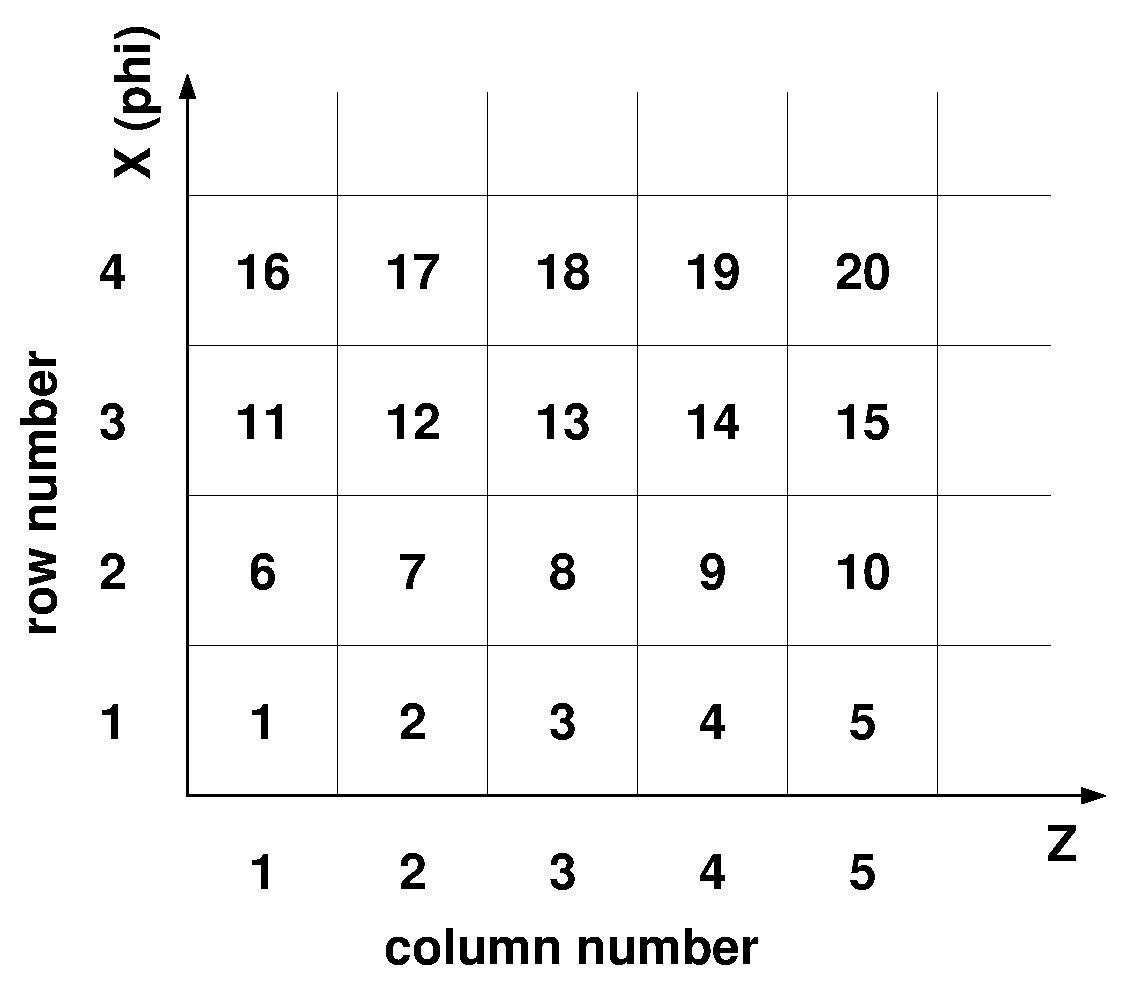
\includegraphics[width=\textwidth]{layout-squarePads.eps}
\end{minipage}}%
\subfigure[MAYA-like layout]{
\begin{minipage}[b]{0.32\textwidth}
\centering
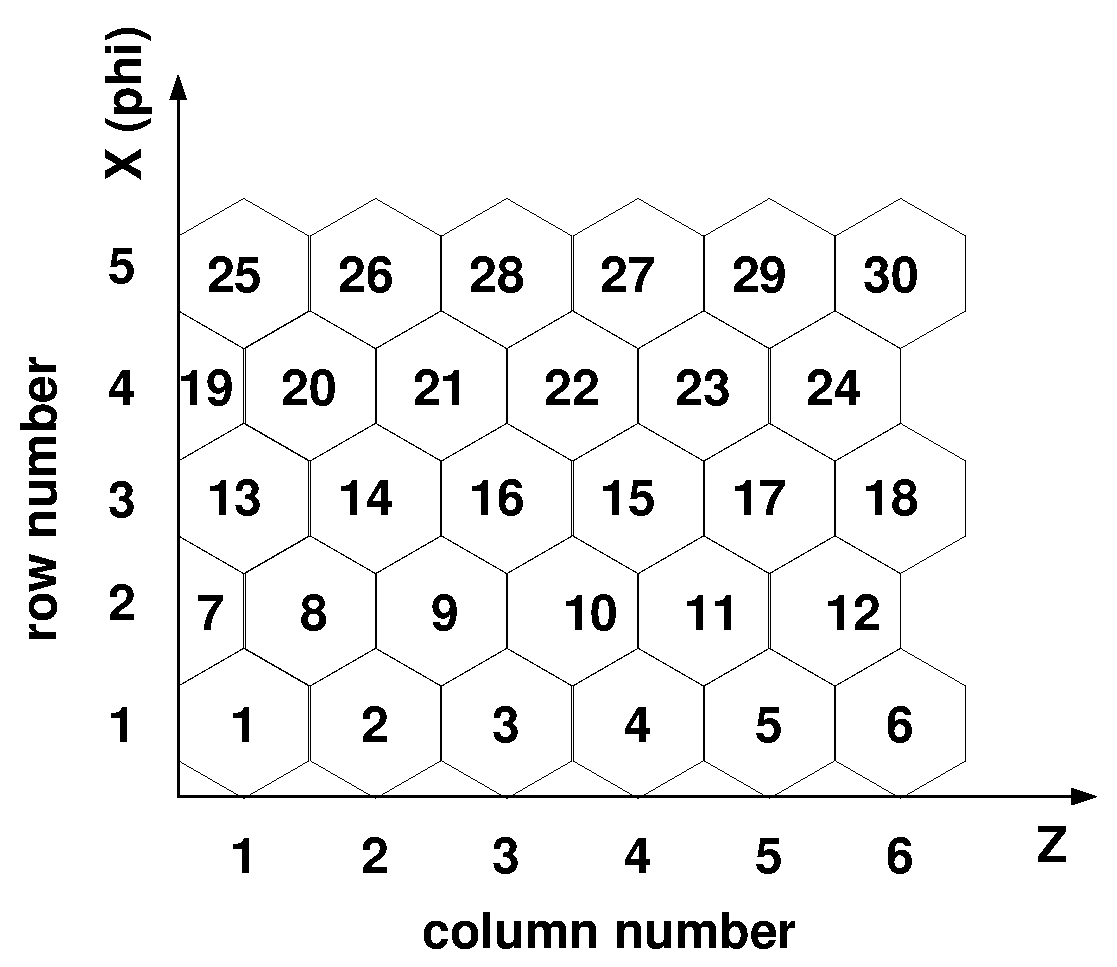
\includegraphics[width=\textwidth]{layout-mayaType.eps}
\end{minipage}}
\subfigure[MAYA-tilted layout]{
\begin{minipage}[b]{0.32\textwidth}
\centering
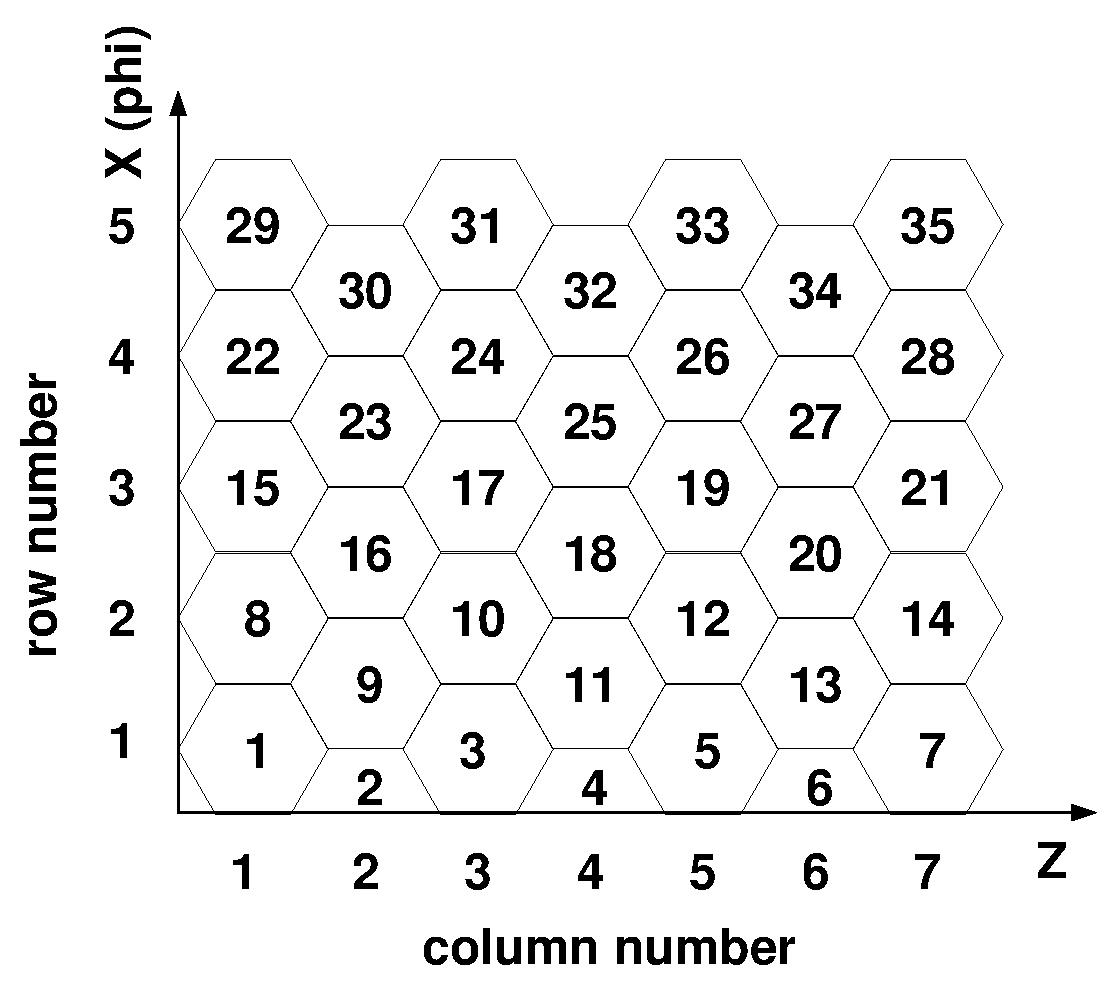
\includegraphics[width=\textwidth]{layout-hexagonal.eps}
\end{minipage}}
\caption{Pad types and layout patterns in the simulation code.}\label{fig-pad-layout}
\end{figure}

In all three cases a single number can identify the pad. The pad number is 1 for row=1, column=1, 2 for row=1, column=2, etc. A set of functions calculates the pad number from the row and column and viceversa.

\subsubsection{Drift velocity and diffusion parameters}
The electron drift velocity\index{drift velocity} and diffusion parameters\index{diffusion parameters} can be passed to the digitizationMacro by using the following commands:
\begin{verbatim}
        theDriftManager.SetDriftVelocity(Double_t velocity)       in mm/ns
        theDriftManager.SetDiffusionParameters(Double_t  long,
                                               Double_t  trans)   in mm^2/ns
\end{verbatim}

For deuterium and isobutane gases, there are analytical formula incorporated in the code to calculate these quantities. To do use these formula, instead of the two commands above, one has to use the following commands instead:
\begin{verbatim}
        theDriftManager.SetDriftParameters(Voltage,height,pressure,gasName)
\end{verbatim}
where, for MAYA-like ACTAR detector, \textit{Voltage} (in volts) is the voltage between the upper cathode and the Frish grid, \textit{height} (in mm) is the distance between the upper cathode and the Frish grid, \textit{pressure} (in mbar) is the pressure of the active gas, and \textit{gasName} is the name of the active gas, it has only two optional values: ``deuterium'' and ``isobutane''. At the end of function \textit{theDriftManager.SetDriftParameters()} the drift velocity and diffusion parameters will be automatically calculated.

The analytical formula for deuterium and isobutane gases were obtained by fitting the corresponding curves in ref.\cite{Peisert-Sauli}. More detailed description of these formula can be found in the \textit{ActarSim-report} by D.Y. Pang.

\subsubsection{Digitization stride-by-stride}
In digitizationMacro, a loop on all events is made for the Tree in the input TFile. Inside each event, a loop on all \textit{ActarSimSimpleTracks} (strides) is performed. For each stride, an object of the class \textit{projectionOnPadPlane} is assigned. This class contains a pointer to the stride, vectors containing the projection on the pad plane for the initial and final points of the stride and the corresponding drift times for each point. Also the values of the longitudinal and transversal sigma of the diffusion distributions is contained.

All this projections and quantities are obtained from the original stride and the geometrical and drift parameters. Actually is the \textit{driftManager} class which calculates them from the original stride using the function:
\begin{verbatim} 
        theDriftManager.CalculatePositionAfterDrift(projection)
\end{verbatim}

Next, the charge induced by the electron drift on the pads is calculated. For this, a candidate pad list is prepared incuding those between the initial and final pads where the projections of the stride lie. A few neighbouring pads are included in the list (by introducing the \textit{securityFactor}) to account for the possible pads diagonal to the initial or final points. Presently, the charge is obtained from the integral of a two dimensional function, which describes the distribution of the induced charges on the pad plane, on the area of the pad (for hexagonal pads, we are using an approximating square limits in the integration -- since it is much more complicated to describe the limits of a hexagonal pad). The form of this function depends on the induction mode (wire, MicroMegas, GEM).
To perform this calculation, the function:
\begin{verbatim}
        theDriftManager.CalculatePadsWithCharge(projection,padSignalCA)
\end{verbatim}
should be called on the event loop.

\subsubsection{The wire induction mode}
In case of wire amplification\index{wire induction mode}, the induced charge distributions, parallel and normal to the wire direction, as a function of the distance between the center of the amplification $x$, are $\rho_1(x)$ and $\rho_2(x)$, respectively. According to the empirical formula of E. Mathieson and J.S. Gordon \cite{Mathieson-NIM-1984, Mathieson-NIMA-1988}, $\rho_1(x)$ and $\rho_2(x)$ are:
\begin{eqnarray}\label{eq-wire-induction}
 \rho(\lambda) &=& q_a\times{}K_1\frac{1-\tanh^2(K_2\lambda)}{1+K_3\tanh^2(K_2\lambda)},\nonumber\\
 K_1 &=& \frac{K_2\sqrt{K_3}}{4\tan^{-1}\sqrt{K_3}},\quad\textrm{and}\\
 K_2 &=& \frac{\pi}{2}\left(1-\frac{\sqrt{K_3}}{2}\right)\nonumber,
\end{eqnarray}
where $q_a$ is the net anode charge, $\lambda=x/h$ with $h$ being the distance between the anode wire plane and the cathode pad plane. To calculate the distributions of induced charge on pads using Eq.(\ref{eq-wire-induction}), the only thing needed is the value of Mathieson factor $K_3$.

The Mathieson factor\index{Mathieson factor} $K_3$ is a function of $r_a/s$ and $h/s$, where $r_a$ and $s$ are radius of the amplification wire and the distance between two neighbouring wires, respectively. Details of calculations of $K_3$ can be found in the \textit{ActarSim-report} by D.Y. Pang. If one want to use wire induction mode, in running of the digitizationMacro, one need to issue the following two commands:
\begin{verbatim}
    theAmplificationManager.SetIsWireOn()
    theAmplificationManager.SetWireAmplificationParameters(0.02,2.,3.)
\end{verbatim}
where the first command switch the wire induction mode on, and the second command passes the wire parameters, $r_a$, $s$ and $h$ to the program (units in mm). In the above example, $r_a=20$ $mu$m, $s=2$ mm and $h=3$ mm, respectively.

\subsubsection{A complete example of running the digitizationMacro}
As explained above, below is one complete example to run the digitizationMacro\index{the digitizationMacro}:
\begin{verbatim}
    $ root -l
    root [0] gSystem->Load("actarsim.sl");
    root [1] .L digitizationMacro.C++
    root [2] thePadsGeometry.SetGeometryValues(0,0,0,150.,150.,150.,100.,2)
    root [3] theDriftManager.SetDriftParameters(10000.,300.,1013.25,"deuterium")
    root [4] theAmplificationManager.SetIsWireOn()
    root [5] theAmplificationManager.SetWireAmplificationParameters(0.02,2.,3.)
    root [6] digitEvents("simData.root","digiData.root",0)
\end{verbatim}
By doing this, we use the digitizationMacro to read the ActarSim output file \textit{simData.root} and write the resulting digitization file into \textit{digiData.root}. The active target ges is deuterium at 1 atm pressure. We are using wire induction mode with wire radius of 0.02 mm, intervals between wires are 2 mm and the wire plane is 3 mm above the pad plane.

\subsection{An example of analyzing macro}
After the digitization, we have the \textit{simulation data} which is equivalent to the experimental data. The simulation data is stored in two file: ancillary detector\index{ancillary detector} signals (silicon and CsI) are stored in the output file of ActarSim (\textit{simData.root}) and pad signals\index{pad signals} (induced charge and time) are stored in the output file of the digitizationMacro (\textit{digiData.root}). Both files are written in a event-by-event way and events related to the same reaction have the same event ID in both files.

In principle, all algorithms developed in the analysis of the MAYA experiment should be able to be applied to the simulation data in the simData.root and digiData.root files. We provide an example macro \textit{analysisExample.C} for this purpose.

For \nuc{78}{Ni} induced $(d,p)$, $(d,d^\prime)$ and $(d,t)$ reactions, the analysisExample macro reconstruct the trajectory\index{trajectory} of the light particle, i.e., proton, deuteron, and triton. From each reaction that the trajectory of the light particle is reconstructable, the analysisExample macro reads the energy signal in silicon and CsI detectors and calculates the range \index{range} of that particle inside the gas. Once the trajectory is known, the $\theta_\text{Lab}$ and $\phi$ angle of the out-going particle in the laboratory system are able to calculated and be compared with their corresponding ``real'' values and then we are able to analysis the angular resolution\index{angular resolution} of the detector for a given gas/pressure, pad information (pad size, shape and pattern of layout), and induction mode. Similarly, the position resolution\index{position resolution} can also be obtained by comparing the reconstructed reaction vertex $Z$-value with its ``real'' value given by Geant4.

To run this macro, the following ROOT command should be used:
\begin{verbatim}
    $ root -l
    root [0] gSystem->Load("actarsim.sl");
    root [1] .L analysisExample.C++
    root [2] thePadsGeometry.SetGeometryValues(0,0,0,150.,150.,150.,100.,2)
    root [3] theDriftManager.SetDriftParameters(10000.,300.,1013.25,"deuterium")
    root [4] reader("simData.root","digiData.root","Ntuples.root",1000.,3,2,0,0,0)
\end{verbatim}

Note that the arguments for functions \textit{SetGeometryValues()} and \textit{SetDriftParameters()} should be the same as the ones used in the corresponding digitizationMacro. The arguments for the function \textit{reader()} are
\begin{enumerate}
 \item simData.root: the output file of ActarSim
 \item digiData.root: the output file of the digitizationMacro
 \item Ntuples.root: the output of this analysisExample macro, in which the following information are stored reaction-by-reaction in a TNtuple\index{ntuple}:
 \begin{itemize}
  \item G4VertexZ: the $Z$-value of the reaction vertex given by Geant4
  \item G4ThetaLab: the $\theta_\text{Lab}$ of the out-going light particle given by Geant4
  \item G4PhiLab: the $\phi$ angle of the out-going light particle given by Geant4
  \item G4VertexE: the beam energy at the reaction vertex given by Geant4 (taking into account the beam energy loss in the gas)
  \item calVertexZ: the $Z$-value of the reaction vertex from the reconstructed particle trajectory
  \item calThetaLab: the $\theta_\text{Lab}$ of the out-going light particle from the reconstructed particle trajectory
  \item calPhiLab: the $\phi$ angle of the out-going light particle from the reconstructed particle trajectory
  \item eSil: the energy loss of the light particle inside the silicon detector (in MeV)
  \item eSci: the energy loss of the light particle inside the CsI detector (in MeV)
  \item protonRangeInGas: the proton range inside the gas (in mm), note that the range is calculated whenever the trajectory of the particle is reconstructable, it does not mean that the particle is stopped inside the gas.
 \end{itemize}

 \item the dynamic range\index{dynamic range}: ratio between the maximum and minimum charge signals that can be measured on the pads. In this analysisExample macro, we determine the minimum charge on the pads by dividing the maximum charge with the dynamic range. This is equivalent to the thresholds\index{thresholds}. In the above example, dynamic range is 1000.

 \item the beam projection width\index{beam projection width} (bw): half of the number of rows of pads that are taken by the beam, the trajectory of light particles is not be able to be reconstructed if its projection on pad plane falles between $[\text{numberOfRows}/2-\text{bw}, \text{numberOfRows}/2+\text{bw}]$. In the above example, bw is 3.

\item the margin width\index{margin width} (mw): number of rows and columns at the edges of the gas chamber. We do not take the signals of the ``margin pads'' as effective singals. In the above example, mw is 2.

\item the last three zeroes in the arguments of the function reader() are verbose level, minimun and maximum reaction numbers (minReactionNumber and maxReactionNumber), respectively. If the verbose level is larger or equal to 1, the program will give some diagnosis information, which is useful if we want to know the details of the running of this macro. If minReactionNumber and maxReactionNumber are zeroes, all reactions will be treated, otherwise, only reactions with reaction number between the minReactionNumber and maxReactionNumber will be treated. In the above example, we include all reactions in the analysis.
\end{enumerate}

In this analysisExample macro, seven histograms\index{histogram} are defined, namely:
\begin{itemize}
\item hLightEvsTheta: two dimensional, $E-\theta_\text{Lab}$ kinematics plot for the out-going light particle, where $E$ are energy signals in ancillary detectors.

\item hDThetavsTheta: two dimensional, $\Delta\theta_\text{Lab}-\theta_\text{Lab}$, this histogram shows how the difference between ``real'' value of $\theta_\text{Lab}$ and its reconstructed value ($\Delta\theta_\text{Lab}$) depends on the value $\theta_\text{Lab}$ itself.

\item hDThetavsPhi: two dimensional, $\Delta\theta_\text{Lab}-\phi$, this histogram shows how $\Delta\theta_\text{Lab}$ depends on the reconstructed $\phi$ value.

\item hRangeVSTheta: two dimensional, correlation between the range of the light particle and its $\theta_\text{Lab}$.

\item hDTheta: one dimensional, angular resolution\index{angular resolution} in $\theta_\text{Lab}$

\item hDPhi: one dimensional, angular resolution in $\phi$

\item hDVertexZ: one dimensional, position resolution\index{position resolution} in reaction vertex $Z$-value.
\end{itemize}

The users of ActarSim can define their own histograms. It is more useful to study the correlations between quantities we are interested in. This can be done by using TNtuples.

\subsection{An example of TNtuple reader}

The analysisExample macro generate an output ROOT file which contains one TNtuple. The contents of this ntuple\index{ntuple} has been introduced in the previous section. We provide the macro \textit{ntupleReader.C} as an example of manipulate these ntuple data members. In this macro we can include as many number of runs of simulation and analysis them together. For example, the $(d,p)$, $(d,d^\prime)$ and $(d,t)$ reactions are simulated in different runs, we can use this macro to put analysis these reactions together.

Some example of the analyzing result using the analysisExample and ntupleReader macros can be find in the \textit{\nuc{78}{Ni}-dp-simulation-report} file by D.Y. Pang.

\section{List of messengers in the Geant4 part of ActarSim}\label{sec-messengers}

Next, a complete description of the possible messenger commands\index{messenger commands} available for selecting different options and for the modification of the behavior of the program. The different messenger commands are ordered and separated by their utility, in different directories. The directories are:
\begin{itemize}
\item \textbf{det:} containing the detector commands\index{detector commands}, able to modify the setup comditions. It contains two subdirectories:  det/sil controlling the Silicon Detectors setup and det/sci controlling the Scintillator Detectors setup.
\item \textbf{phys:} containing all related with the interaction physics\index{interaction physics};
\item \textbf{gun:} commands related with the event generation\index{event generation};
\item \textbf{event:} event visualization\index{visualization};
\item \textbf{analControl:} histogramming control\index{histogramming control}.
\end{itemize}

For each case, the command complete name initiates the description, following by the command explanation and some additional features, if required.

\subsection{Commands controlling the detector description:}
\index{detector commands}
\begin{verbatim}
/ActarSim/det/
        Command description.  Just the directory name...

/ActarSim/det/gasGeoIncludedFlag
        Includes the geometry of the gas volume in the simulation (default "off").

/ActarSim/det/silGeoIncludedFlag
        Includes the geometry of the silicons in the simulation (default "off").

/ActarSim/det/sciGeoIncludedFlag
        Includes the geometry of the scintillator in the simulation (default "off").

/ActarSim/det/setMediumMat
        Select Material of the Medium.

/ActarSim/det/setEleField
        Define electric field.
        Usage: /ActarSim/det/setEleField  Ex  Ey  Ez  (in MV/mm)

/ActarSim/det/setMagField
        Define magnetic field.
        Usage: /ActarSim/det/setMagField  Bx  By  Bz  unit

/ActarSim/det/update
        Update geometry.
        This command MUST be applied before \"beamOn\"
        if you changed geometrical value(s) or gas density.

/ActarSim/det/print
        Prints geometry.
\end{verbatim}
 
\subsubsection{gas box detector commands}
 \index{detector commands}
\begin{verbatim}
/ActarSim/det/setGasMat
        Select Material of the Gas.
        DefaultValue("isoC4H10")

/ActarSim/det/gas/setBeamShieldMat
        Select Material of the beam shield.
        DefaultValue("isoC4H10")

/ActarSim/det/gas/setDetectorGeometry
        Select the geometry of the detector.
        DefaultValue("box")

/ActarSim/det/gas/setBeamShield
        Sets a beam shield and selects the geometry.
        DefaultValue("tube")

/ActarSim/det/gas/setBeamShieldMat
        Select Material of the beam shield.
        DefaultValue("isoC4H10")

/ActarSim/det/gas/setXLengthGasBox
        Select the half-length X dimension of the Gas Box

/ActarSim/det/gas/setYLengthGasBox
        Select the half-length Y dimension of the Gas Box

/ActarSim/det/gas/setZLengthGasBox
        Select the half-length Z dimension of the Gas Box

/ActarSim/det/gas/setRadiusGasTub
        Select the external radius of the Gas Tube.

/ActarSim/det/gas/setLengthGasTub
        Select the half-length of the Gas Tube.

/ActarSim/det/gas/setInnerRadiusBeamShieldTub
        Select the external radius of the Gas Tube.

/ActarSim/det/gas/setRadiusBeamShieldTub
        Select the internal radius of the Gas Tube.

/ActarSim/det/gas/setLengthBeamShieldTub
        Select the half-length of the Gas Tube.

/ActarSim/det/gas/print
        Prints geometry.
\end{verbatim}

\subsubsection{silicon detector commands}
\index{detector commands}
\begin{verbatim}
/ActarSim/det/sil/
        Silicon detector control

/ActarSim/det/sil/print
        Prints geometry.

/ActarSim/det/sil/sideCoverage
        Selects the silicon coverage (default 1).
        6 bits to indicate which sci wall is present (1) or absent (0).
        The order is:
        bit1 (lsb) beam output wall
        bit2 lower (gravity based) wall
        bit3 upper (gravity based) wall
        bit4 left (from beam point of view) wall
        bit5 right (from beam point of view) wall
        bit6 (msb) beam entrance wall
        Convert the final binary to a decimal number and set the coverage!

/ActarSim/det/sil/xBoxHalfLength
        Sets the x half length of the silicon detectors box
        DefaultValue(0.5)

/ActarSim/det/sil/yBoxHalfLength
        Sets the y half length of the silicon detectors box
        DefaultValue(0.5)

/ActarSim/det/sil/zBoxHalfLength
        Sets the z half length of the silicon detectors box
        DefaultValue(0.5)
\end{verbatim}

\subsubsection{scintillator detector commands}
\index{detector commands}
\begin{verbatim}
/ActarSim/det/sci/
        Scintillator detector control

/ActarSim/det/sci/print
        Prints geometry.

/ActarSim/det/sci/sideCoverage
        Selects the scintillator coverage (default 1).
        6 bits to indicate which sci wall is present (1) or absent (0).
        The order is:
        bit1 (lsb) beam output wall
        bit2 lower (gravity based) wall
        bit3 upper (gravity based) wall
        bit4 left (from beam point of view) wall
        bit5 right (from beam point of view) wall
        bit6 (msb) beam entrance wall
        Convert the final binary to a decimal number and set the coverage!

/ActarSim/det/sci/xBoxHalfLength
        Sets the x half length of the scintillator detectors box
        DefaultValue(0.5)

/ActarSim/det/sci/yBoxHalfLength
        Sets the y half length of the scintillator detectors box
        DefaultValue(0.5)

/ActarSim/det/sci/zBoxHalfLength
        Sets the z half length of the scintillator detectors box
        DefaultValue(0.5)
\end{verbatim}

\textbf{IMPORTANT NOTE}: \textit{/ActarSim/det/update} should be called after each geometrycal modification. This command MUST be applied before \textit{/run/beamOn}.

Note: the geometries of sil and sci detectors are hard-coded right now, it should be modified to cope with different setups and possibilities.

\subsection{physics processes commands}
\index{interaction physics}
The full bank of particles  (ConstructBosons(); ConstructLeptons(); ConstructMesons(); ConstructBaryons(); G4ShortLivedConstructor and
G4IonConstructor) are constructed. The physics processes (transportation, em and decay) are now taken from the \textit{examples/extended/medical/GammaTherapy} (basically the PhysicsList implementation for em processes). Other hadronic particles are proccesses are also taken from this example. Note that the PhysicsList can be selected between several possibilities:

\begin{verbatim}
             em: standard, lowenergy, penelope, (choose one from these three)
         common: decay
       hadronic: elastic, binary, binary_ion, gamma_nuc
 ion low-energy: ion-LowE, ion-LowE-ziegler1977, ion-LowE-ziegler1985,
                 ion-LowE-ziegler2000, ion-standard
\end{verbatim}

\begin{verbatim}
/ActarSim/phys/
        Physics list commands directory

/ActarSim/phys/setGCut
        Set gamma cut.

/ActarSim/phys/setECut
        Set electron cut.

/ActarSim/phys/setPCut
        Set positron cut.

/ActarSim/phys/setCuts
        Set cut for all.

/ActarSim/phys/addPhysics
        Add modula physics list.

/ActarSim/phys/verbose
        Set verbose level for processes
\end{verbatim}

Note that a \textit{/run/initialization} is now needed to initialize the application. This initialization has been removed from the \textit{ActarSim.cc} main function to permit the definition of different physics (lowenergy, penelope...) from the PhysicsList before the initialization. An example of how to initialize is shown in the macros (test1.mac, for instance).

\subsection{event generation commands}

The event generation\index{event generation} can be controled by user commands under the directory \textit{/ActarSim/gun} and subdirectories inside. There are several types of reactions that the program handles:

\begin{verbatim}
A) Track a particle or set of particles defined from the Particles list. 
This mode is selected setting the commands 
        /ActarSim/gun/reactionFromFile off (default behavior)
        /ActarSim/gun/reactionFromCine off 
        ...
B) Track a predefined reaction from a file 
C) Track a reaction calculated from CINE (program from W. Mittig)
D) Track a reaction calculated from KINE (program from M.S. Golovkov)
\end{verbatim}

For each case, a realistic interaction (beam distribution and interaction over all gas volume, plus the energy lost of the beam in the gas before the reaction). These commands are described below:

\begin{verbatim}
/ActarSim/gun/realisticBeam
        Simulates beam emittance according to emittance parameters.
         Choice : on, off(default)

/ActarSim/gun/beamInteraction
        Simulates the beam energy loss in gas.
         Choice : on, off(default)

/ActarSim/gun/emittance
        Selects the value of the emittance [in mm mrad].  
        Default value is 1 mm mrad. 

/ActarSim/gun/beamRadiusAtEntrance
        Selects the beam radius at entrance of ACTAR.
        Used with the emittance to calculate the position and angle
          distributions of the beam when a realisticBeam option is set.
\end{verbatim}

\subsubsection{Track a particle or set of particles defined from the Particles list}

\begin{verbatim}
/ActarSim/gun/List
        List available particles. Invoke G4ParticleTable.

/ActarSim/gun/particle
        Select the incident particle (proton is default)
        (ion can be specified for shooting ions).

/ActarSim/gun/ion
        Set properties of ion to be generated.
        [usage] /gun/ion Z A Q E
                Z:(int) AtomicNumber
                A:(int) AtomicMass
                Q:(int) Charge of Ion (in unit of e)
                E:(double) Excitation energy (in keV)

/ActarSim/gun/energy
        Sets the kinetic energy of the primary particle
        DefaultValue(20.)

/ActarSim/gun/direction
        Set momentum direction.
        Direction needs not to be a unit vector.

/ActarSim/gun/position
        Set starting position of the particle.

/ActarSim/gun/time      
        Set initial time of the particle.

/ActarSim/gun/polarization
        Set polarization.

/ActarSim/gun/number
        Set number of particles to be generated.

/ActarSim/gun/randomVertexZPosition on
        Set the vertex Z-value random or not
        Choice: on (default), off

/ActarSim/gun/randomVertexZRange min max unit
        This command is effective only if randomVertexZPosition=="on"
        min: minimum vertex Z-value, default: 0
        max: maximum vertex Z-value, default: 300
        unit: defaule mm

/ActarSim/gun/vertexZPosition z-value unit
        This command if effective only if randomVertexZPosition=="off"
        z-value: user-given vertex Z-value
        unit: default mm
\end{verbatim}


\subsubsection{Track a predefined reaction from a file}

\begin{verbatim}
/ActarSim/gun/reactionFromFile
        Select a reaction from an input file
        Choice : on, off(default)

/ActarSim/gun/reactionFile
        Select the reaction definition file
\end{verbatim}


\subsubsection{Track a reaction calculated from CINE (program from W. Mittig)}
\index{CINE}
\begin{verbatim}
/ActarSim/gun/reactionFromCine
        Select a reaction using Cine
        Choice : on, off(default)

Note that the following commands are under the subdirectory Cine

/ActarSim/gun/Cine/randomTheta
        Select a random Theta angle for the scattered particle.
        Choice : on(default), off

/ActarSim/gun/Cine/randomThetaVal
        Sets the limit in the Theta angle for the scattered particle.
        The value is randomly chosen between the limits (degrees)
               [usage] /ActarSim/gun/Cine/incidentIon min max 
                min: the minimum angle (default 0 degrees)
                        max: the maximum angle (default 180 degrees)

/ActarSim/gun/Cine/thetaLabAngle        
        Sets theta lab angle for the scattered particle (degrees)
        DefaultValue(0.5)

/ActarSim/gun/Cine/incidentIon
        Set properties of incident ion to be generated.
        [usage] /ActarSim/gun/Cine/incidentIon Z A Q E
                Z:(int) AtomicNumber
                A:(int) AtomicMass
                Q:(int) Charge of ion (in unit of e)
                E:(double) Excitation energy (in keV)

/ActarSim/gun/Cine/targetIon
        Set properties of target ion to be generated.
        [usage] /ActarSim/gun/Cine/targetIon Z A Q E
                Z:(int) AtomicNumber
                A:(int) AtomicMass
                Q:(int) Charge of ion (in unit of e)
                E:(double) Excitation energy (in keV)

/ActarSim/gun/Cine/scatteredIon
        Set properties of scattered ion to be generated.
        [usage] /ActarSim/gun/Cine/scatteredIon Z A Q E
                Z:(int) AtomicNumber
                A:(int) AtomicMass
                Q:(int) Charge of ion (in unit of e)
                E:(double) Excitation energy (in keV)

/ActarSim/gun/Cine/recoilIon
        Set properties of recoil ion to be generated.
        [usage] /ActarSim/gun/Cine/recoilIon Z A Q E
                Z:(int) AtomicNumber
                A:(int) AtomicMass
                Q:(int) Charge of ion (in unit of e)
                E:(double) Excitation energy (in keV)

/ActarSim/gun/Cine/reactionQ  
        Sets the reaction Q-value for the ground state (MeV)

/ActarSim/gun/Cine/labEnergy
        Sets the laboratory energy (MeV)
\end{verbatim}

\subsubsection{Track a reaction calculated from KINE (program from M.S. Golovkov)}
\index{KINE}
\begin{verbatim}
/ActarSim/gun/reactionFromKine
        Select a reaction using KINE
        Choice : on(default), off

Note that the following commands are under the subdirectory Kine

/ActarSim/gun/Kine/randomTheta
    Select a random Theta angle for the scattered particle.
    Choice : on(default), off

/ActarSim/gun/Kine/randomThetaVal
    Set the range of theta angles if it is to be randomly chosen
    [usage] /ActarSim/gun/Kine/randomThetaVal min, max
            min: the minimum angle (default 0 degrees)
            max: the maximum angle (default 180 degrees)

/ActarSim/gun/Kine/incidentIon
    Set the properties of the incident ion
    [usage] /ActarSim/gun/Kine/incidentIon Z A Q Ex Mass
            Z: atomic number (I)
            A: mass number   (I)
            Q: charge number (I)
           Ex: excitation energy (D, in MeV)
         Mass: mass (D, in u)  

/ActarSim/gun/Kine/targetIon
    Set the properties of the target ion
    [usage] /ActarSim/gun/Kine/targetIon Z A Q Ex Mass
            Z: atomic number (I)
            A: mass number   (I)
            Q: charge number (I)
           Ex: excitation energy (D, in MeV)
         Mass: mass (D, in u)  

/ActarSim/gun/Kine/scatteredIon
    Set the properties of the scattered ion
    [usage] /ActarSim/gun/Kine/scatteredIon Z A Q Ex Mass
            Z: atomic number (I)
            A: mass number   (I)
            Q: charge number (I)
           Ex: excitation energy (D, in MeV)
         Mass: mass (D, in u)  

/ActarSim/gun/Kine/recoilIon
    Set the properties of the recoiled ion
    [usage] /ActarSim/gun/Kine/recoilIon Z A Q Ex Mass
            Z: atomic number (I)
            A: mass number   (I)
            Q: charge number (I)
           Ex: excitation energy (D, in MeV)
         Mass: mass (D, in u)  

/ActarSim/gun/Kine/labEnergy
    Set the incident energy
    [usage] /ActarSim/gun/Kine/labEnergy E MeV
            E: incident energy (D)
          MeV: the unit

/ActarSim/gun/Kine/randomThetaCM
    Randomize or not the Theta_cm value
    Choice: on (default), off
    Default: on

/ActarSim/gun/Kine/randomThetaRange min max unit
    This command is effective only if randomThetaCM=="on"
    min: default value 0.
    max: default value 180.
    unit: default deg

/ActarSim/gun/Kine/randomPhiAngle
    Randomize or not the Phi angle, useful when testing analyzing macros
    Choice: on (default), off
    default: on

/ActarSim/gun/Kine/userThetaCM theta_cm unit
    This command is effective only if randomThetaCM is "off"
    theta_cm: user given Theta_cm for KINE
    unit: default deg

/ActarSim/gun/Kine/userPhiAngle Phi unit
    This command is effective only if randomPhiAngle is "off"
    Phi: user given phi angle of the recoiled particle,
         e.g., proton in the 78Ni(d,p)79Ni reaction in inverse kinematics
    unit: default deg
\end{verbatim}

\subsection{event visualization}

Inside the \textit{ActarSimEventAction} one can chose the visualization\index{visualization} of the tracks in the event, in particular the user command:

\begin{verbatim}
/ActarSim/event/drawTracks
        Draw the tracks in the event (Choice : none, charged, neutral, all(default))
        DefaultValue("all");

/ActarSim/event/printModulo
        Print events (modulo n, that is prints every n event)
\end{verbatim}

\subsection{histogramming control}

The Tree and histograms\index{histogramming control} can be controled by user commands under the directory \textit{/ActarSim/analControl} and subdirectories inside:

\begin{verbatim}
/ActarSim/analControl/storeTracks
        Store the tracks in the output Tree
        Choice : on, off(default)

/ActarSim/analControl/storeTrackHistos
        Store the tracks in Histograms
        Choice : on, off(default)

/ActarSim/analControl/storeEvents
        Store the events in the output Tree
        DefaultValue("off")

/ActarSim/analControl/storeSimpleTracks
        Store the simple tracks in the output Tree
        DefaultValue("off")

/ActarSim/analControl/storeHistograms
        Store the events in the output Tree
        Choice : on, off(default)
\end{verbatim}

\section{Appendix}

\subsection{An example of macro for ActarSim}\label{sec-ActarSim-macro}
This macro simulates 5000 \nuc{78}{Ni}(d,p)\nuc{79}{Ni} reactions at 8 AMeV with \nuc{79}{Ni} at an excited state of 5 MeV.

\begin{verbatim}
################################################################
#*-- AUTHOR : Hector Alvarez-Pol
#*-- Date: 05/2005
#*-- Last Update: 15/05/08
#*-- Copyright: GENP (Univ. Santiago de Compostela)
# --------------------------------------------------------------
# Comments:
#     - 15/05/08 Multidetector geometry
#     - 05/05/06 Updating to new ActarSim (geant4.8) code
#     - 22/11/05 Updated including CINE options
#     - 31/05/05 Macro for ACTAR simulation
#
################################################################
# Macro file for testing online jobs
################################################################
# verbosity levels and saveHistory
/control/verbose 0
/control/saveHistory
/run/verbose 0
/event/verbose 0
/tracking/verbose 0
#
# Setting the Physics modules; valid values are here listed:
#   em: standard, lowenergy, penelope, (choose one from this three)
#   common: decay,
#   hadronic: elastic, binary, binary_ion, gamma_nuc,
#   ion low-energy: ion-LowE, ion-LowE-ziegler1977, ion-LowE-ziegler1985,
#   ion-LowE-ziegler2000, ion-standard
#
/ActarSim/phys/addPhysics standard
#/ActarSim/phys/addPhysics decay
#/ActarSim/phys/addPhysics elastic
#/ActarSim/phys/addPhysics binary
#/ActarSim/phys/addPhysics binary_ion
#/ActarSim/phys/addPhysics gamma_nuc
#/ActarSim/phys/addPhysics lowenergy
#/ActarSim/phys/addPhysics ion-LowE
#/ActarSim/phys/addPhysics ion-LowE-ziegler1977
#/ActarSim/phys/addPhysics ion-LowE-ziegler1985
#/ActarSim/phys/addPhysics ion-LowE-ziegler2000
#/ActarSim/phys/addPhysics ion-standard
#/ActarSim/phys/addPhysics penelope
#
# Cuts for the particles  (incomplete list, see README)
#
#  /ActarSim/phys/setGCut 0.1
#  /ActarSim/phys/setECut 0.1
#  /ActarSim/phys/setPCut 0.1
#  /ActarSim/phys/setCuts 0.1
/ActarSim/phys/verbose 0
#
# Initialization is moved here from the main allowing PhysicsList
#
/run/initialize
#
# DETECTOR CHARACTERIZATION
#
# GENERAL COMMANDS
#
# Control of the materials
/ActarSim/det/setMediumMat Galactic
#Electric and Magnetic fields
/ActarSim/det/setEleField 0 0 0
/ActarSim/det/setMagField 0 0 0 T
#
# GAS DETECTOR
#
/ActarSim/det/gasGeoIncludedFlag on
# if box
/ActarSim/det/gas/setDetectorGeometry box
/ActarSim/det/gas/setXLengthGasBox 150. mm
/ActarSim/det/gas/setYLengthGasBox 150. mm
/ActarSim/det/gas/setZLengthGasBox 150. mm
#
# if tube
#  /ActarSim/det/gas/setDetectorGeometry tube
#  /ActarSim/det/gas/setRadiusGasTub 1.0 cm
#  /ActarSim/det/gas/setLengthGasTub 1.0 cm
#
# Beam shield? tube or off
/ActarSim/det/gas/setBeamShield off
#  /ActarSim/det/gas/setBeamShield on
#  /ActarSim/det/gas/setBeamShieldMat Ion
#  /ActarSim/det/gas/setInnerRadiusBeamShieldTub 1.0 mm
#  /ActarSim/det/gas/setRadiusBeamShieldTub 1.001 mm
#  /ActarSim/det/gas/setLengthBeamShieldTub 1.0 m
#
# gas material: isoC4H10STP,  isoC4H10_150, isoC4H10_220,
#               isoC4H10_300, isoC4H10_500, isoC4H10_710,
#               isoC4H10_1300,isoC4H10_1880
#               D2_40, D2_60, D2_80, D2_100, to D2_400 with steps of 20 mbar
#               D2_STP, D2_1695, D2_1800, D2_1950
#               He_1900, He_2010
#
/ActarSim/det/gas/setGasMat D2_STP
#
# SILICON DETECTOR
#
/ActarSim/det/silGeoIncludedFlag on
#Options for Silicon and scintillator coverage:
# 6 bits to indicate which sci wall is present (1) or absent (0)
# order is:
# bit1 (lsb) beam output wall                 1
# bit2 lower (gravity based) wall             2
# bit3 upper (gravity based) wall             4
# bit4 left (from beam point of view) wall    8
# bit5 right (from beam point of view) wall   16
# bit6 (msb) beam entrance wall               32
# examples: 63 full coverage; 3 only output and bottom walls ...
/ActarSim/det/sil/sideCoverage 56
/ActarSim/det/sil/xBoxHalfLength 150. mm
/ActarSim/det/sil/yBoxHalfLength 150. mm
/ActarSim/det/sil/zBoxHalfLength 150. mm
/ActarSim/det/sil/print
#
# SCINTILLATOR DETECTOR
#
/ActarSim/det/sciGeoIncludedFlag on
# see above explanation in the equivalent command for the Silicons
/ActarSim/det/sci/sideCoverage 56
/ActarSim/det/sci/xBoxHalfLength 150. mm
/ActarSim/det/sci/yBoxHalfLength 150. mm
/ActarSim/det/sci/zBoxHalfLength 150. mm
/ActarSim/det/sci/print
#
#Control of the output on the ROOT file
#all the tracks are stored (note: huge space comsumption)
#Note: it should come before the update!!!
/ActarSim/analControl/storeTracks off
/ActarSim/analControl/storeTrackHistos off
/ActarSim/analControl/storeEvents on
/ActarSim/analControl/storeHistograms off
/ActarSim/analControl/storeSimpleTracks on
#/ActarSim/analControl/setMinStrideLength 0.1
#
# Update is mandatory after any material,field or detector change
#
/ActarSim/det/update
/ActarSim/det/print
#
# Control of the primary events
#For all cases the possibility to have realistic beam distribution
/ActarSim/gun/beamInteraction on
/ActarSim/gun/realisticBeam on
/ActarSim/gun/beamRadiusAtEntrance 2.5 mm
/ActarSim/gun/emittance 200.0
#
# Realistic Event-Generator on
/ActarSim/gun/reactionFromEvGen off
#
# Reaction from Cine and Event-Generator
/ActarSim/gun/reactionFromCine off
/ActarSim/gun/reactionFromCrossSection off
#
# A) Track a particle or set of particles defined from the Particles list
#
#/ActarSim/gun/List
#/ActarSim/gun/particle proton
#if you want to use an ion, write "ion" in the previous command
#and set the Z, A and charge state in the next...
#/ActarSim/gun/ion 3 11 3
#/ActarSim/gun/energy 11. MeV
#/ActarSim/gun/direction 0 0 1
#/ActarSim/gun/time 0
#/ActarSim/gun/polarization 0
#/ActarSim/gun/number 1
/ActarSim/gun/randomVertexZPosition on
/ActarSim/gun/randomVertexZRange 145. 155. mm
/ActarSim/gun/vertexZPosition 2.0 cm
#
#
# B) Track a predefined reaction from a file:
#
/ActarSim/gun/reactionFromFile off
#if you select a reaction, you should say the file in the command below
#possibilities are (up to now): He8onp_100MeV_Elastic.dat,
#He8onp_100MeV_tritium.dat, He8onC12_100MeV_Elastic.dat,
#He8onp_50MeV_Elastic.dat, He8onC12_50MeV_Elastic.dat, He8onp_50MeV_tritium.dat
#
#/ActarSim/gun/reactionFile /data/He8onp_50MeV_Elastic.dat
#/ActarSim/gun/randomReaction off    STILL NOT DONE -- ALWAYS RANDOM
#/ActarSim/gun/rowInFileReaction 4   STILL NOT DONE -- ALWAYS RANDOM
#
#C) Track a reacion calculated from CINE (program from W. Mittig)
#
/ActarSim/gun/reactionFromCine off
#/ActarSim/gun/Cine/incidentIon 3 8 3 0.0
#/ActarSim/gun/Cine/targetIon 2 4 2 0.0
#/ActarSim/gun/Cine/scatteredIon 3 8 3 1.0
#/ActarSim/gun/Cine/recoilIon 2 4 2 0.0
#/ActarSim/gun/Cine/reactionQ 1. MeV
#/ActarSim/gun/Cine/labEnergy 70 MeV
#/ActarSim/gun/Cine/randomTheta on
#/ActarSim/gun/Cine/thetaLabAngle 0.1
#
#D) Track a reacion calculated from KINE
#
/ActarSim/gun/reactionFromKine on
/ActarSim/gun/Kine/incidentIon 28 78 28 0.0 77.96318
/ActarSim/gun/Kine/targetIon 1 2 1 0.0 2.0141
/ActarSim/gun/Kine/scatteredIon 28 79 28 5.0 78.97107
/ActarSim/gun/Kine/recoilIon 1 1 1 0.0 1.007825
/ActarSim/gun/Kine/labEnergy 624. MeV
/ActarSim/gun/Kine/randomThetaCM on
/ActarSim/gun/Kine/randomThetaRange 0.0 180.0
/ActarSim/gun/Kine/randomPhiAngle on
/ActarSim/gun/Kine/userThetaCM 41.0 deg
/ActarSim/gun/Kine/userPhiAngle 50.0 deg
#
# VISUALIZATION
#
# Draw the whole geometry tree with details as function of verbosity
#   /vis/ASCIITree/verbose 10
#   /vis/drawTree
# visualization
#   /vis/scene/create
#   /vis/open OGLIX
#   /vis/viewer/set/autoRefresh 0
#/vis/viewer/flush
# set camera
#   /vis/viewer/reset
#   /vis/viewer/set/hiddenEdge 1
#   /vis/viewer/set/lightsThetaPhi 120 40
#/vis/viewer/set/viewpointThetaPhi 115. 145.
#   /vis/viewer/set/viewpointThetaPhi 90. 90.
#   /vis/viewer/zoom 1.0
#   /vis/viewer/set/background 1 1 1 1
#/vis/viewer/flush
#
# drawing style
#   /vis/viewer/set/style surface
#/vis/viewer/set/style wireframe
#/vis/viewer/flush
#
# drawing the tracks
#   /tracking/storeTrajectory 1
#   /vis/scene/endOfEventAction accumulate
#   /vis/viewer/set/autoRefresh 1
#
# create an empty scene and add the detector geometry to it
#/vis/drawVolume
#/vis/scene/add/axes 0 0 0 0.1 m
#/ActarSim/event/drawTracks all
#/ActarSim/event/printModulo 1
#
# RUN: number of events
#
/run/beamOn 10002
\end{verbatim}



\printindex

\begin{thebibliography}{999}
\bibitem{Peisert-Sauli} Anna Peisert and Fabio Sauli, Drift and Diffusion of electrons in gases: a compilation, CERN 84-08, 1984
\bibitem{Mathieson-NIM-1984} E. Mathieson and J.S. Gordon, Nucl. Instru. Meth. 227 (1984) 277.
\bibitem{Mathieson-NIMA-1988} E. Mathieson, Nucl. Instru. Meth. \textbf{A270} (1988) 602.
\end{thebibliography}

\end{document}